\section{Mathematical model and numerical experiments}
\label{model}

A detailed formulation will be described here.

\begin{displaymath}
-C_{\rm m} \frac{dV_{\rm m}}{dt} = I_{\rm Na_b} + I_{\rm K_b}
                               + I_{\rm NaK} + I_{\rm NaCa}
                               + \textcolor{missing}{I_{\rm NaH}} + I_{\rm K_{ur}}
                               + \textcolor{missing}{I_{\rm K_{2\, pore}}}
                               + \textcolor{missing}{I_{\rm Ca_{act}K}}
                               + I_{\rm TRP} + I_{\rm stim}
\end{displaymath}
\centering
% GNUPLOT: LaTeX picture with Postscript
\begingroup
  \makeatletter
  \providecommand\color[2][]{%
    \GenericError{(gnuplot) \space\space\space\@spaces}{%
      Package color not loaded in conjunction with
      terminal option `colourtext'%
    }{See the gnuplot documentation for explanation.%
    }{Either use 'blacktext' in gnuplot or load the package
      color.sty in LaTeX.}%
    \renewcommand\color[2][]{}%
  }%
  \providecommand\includegraphics[2][]{%
    \GenericError{(gnuplot) \space\space\space\@spaces}{%
      Package graphicx or graphics not loaded%
    }{See the gnuplot documentation for explanation.%
    }{The gnuplot epslatex terminal needs graphicx.sty or graphics.sty.}%
    \renewcommand\includegraphics[2][]{}%
  }%
  \providecommand\rotatebox[2]{#2}%
  \@ifundefined{ifGPcolor}{%
    \newif\ifGPcolor
    \GPcolortrue
  }{}%
  \@ifundefined{ifGPblacktext}{%
    \newif\ifGPblacktext
    \GPblacktexttrue
  }{}%
  % define a \g@addto@macro without @ in the name:
  \let\gplgaddtomacro\g@addto@macro
  % define empty templates for all commands taking text:
  \gdef\gplbacktext{}%
  \gdef\gplfronttext{}%
  \makeatother
  \ifGPblacktext
    % no textcolor at all
    \def\colorrgb#1{}%
    \def\colorgray#1{}%
  \else
    % gray or color?
    \ifGPcolor
      \def\colorrgb#1{\color[rgb]{#1}}%
      \def\colorgray#1{\color[gray]{#1}}%
      \expandafter\def\csname LTw\endcsname{\color{white}}%
      \expandafter\def\csname LTb\endcsname{\color{black}}%
      \expandafter\def\csname LTa\endcsname{\color{black}}%
      \expandafter\def\csname LT0\endcsname{\color[rgb]{1,0,0}}%
      \expandafter\def\csname LT1\endcsname{\color[rgb]{0,1,0}}%
      \expandafter\def\csname LT2\endcsname{\color[rgb]{0,0,1}}%
      \expandafter\def\csname LT3\endcsname{\color[rgb]{1,0,1}}%
      \expandafter\def\csname LT4\endcsname{\color[rgb]{0,1,1}}%
      \expandafter\def\csname LT5\endcsname{\color[rgb]{1,1,0}}%
      \expandafter\def\csname LT6\endcsname{\color[rgb]{0,0,0}}%
      \expandafter\def\csname LT7\endcsname{\color[rgb]{1,0.3,0}}%
      \expandafter\def\csname LT8\endcsname{\color[rgb]{0.5,0.5,0.5}}%
    \else
      % gray
      \def\colorrgb#1{\color{black}}%
      \def\colorgray#1{\color[gray]{#1}}%
      \expandafter\def\csname LTw\endcsname{\color{white}}%
      \expandafter\def\csname LTb\endcsname{\color{black}}%
      \expandafter\def\csname LTa\endcsname{\color{black}}%
      \expandafter\def\csname LT0\endcsname{\color{black}}%
      \expandafter\def\csname LT1\endcsname{\color{black}}%
      \expandafter\def\csname LT2\endcsname{\color{black}}%
      \expandafter\def\csname LT3\endcsname{\color{black}}%
      \expandafter\def\csname LT4\endcsname{\color{black}}%
      \expandafter\def\csname LT5\endcsname{\color{black}}%
      \expandafter\def\csname LT6\endcsname{\color{black}}%
      \expandafter\def\csname LT7\endcsname{\color{black}}%
      \expandafter\def\csname LT8\endcsname{\color{black}}%
    \fi
  \fi
  \setlength{\unitlength}{0.0324bp}%
  \begin{picture}(11520.00,8640.00)%
    \gplgaddtomacro\gplbacktext{%
      \colorrgb{0.00,0.00,0.00}%
      \put(1365,950){\makebox(0,0)[r]{\strut{}-86.4}}%
      \colorrgb{0.00,0.00,0.00}%
      \put(1365,2124){\makebox(0,0)[r]{\strut{}-86.2}}%
      \colorrgb{0.00,0.00,0.00}%
      \put(1365,3297){\makebox(0,0)[r]{\strut{}-86}}%
      \colorrgb{0.00,0.00,0.00}%
      \put(1365,4471){\makebox(0,0)[r]{\strut{}-85.8}}%
      \colorrgb{0.00,0.00,0.00}%
      \put(1365,5644){\makebox(0,0)[r]{\strut{}-85.6}}%
      \colorrgb{0.00,0.00,0.00}%
      \put(1365,6818){\makebox(0,0)[r]{\strut{}-85.4}}%
      \colorrgb{0.00,0.00,0.00}%
      \put(1365,7991){\makebox(0,0)[r]{\strut{}-85.2}}%
      \colorrgb{0.00,0.00,0.00}%
      \put(1497,730){\makebox(0,0){\strut{}0}}%
      \colorrgb{0.00,0.00,0.00}%
      \put(2613,730){\makebox(0,0){\strut{}0.5}}%
      \colorrgb{0.00,0.00,0.00}%
      \put(3729,730){\makebox(0,0){\strut{}1}}%
      \colorrgb{0.00,0.00,0.00}%
      \put(4845,730){\makebox(0,0){\strut{}1.5}}%
      \colorrgb{0.00,0.00,0.00}%
      \put(5961,730){\makebox(0,0){\strut{}2}}%
      \colorrgb{0.00,0.00,0.00}%
      \put(7076,730){\makebox(0,0){\strut{}2.5}}%
      \colorrgb{0.00,0.00,0.00}%
      \put(8192,730){\makebox(0,0){\strut{}3}}%
      \colorrgb{0.00,0.00,0.00}%
      \put(9308,730){\makebox(0,0){\strut{}3.5}}%
      \colorrgb{0.00,0.00,0.00}%
      \put(10424,730){\makebox(0,0){\strut{}4}}%
      \colorrgb{0.00,0.00,0.00}%
      \put(463,4470){\rotatebox{90}{\makebox(0,0){\strut{}Membrane voltage (mV)}}}%
      \colorrgb{0.00,0.00,0.00}%
      \put(5960,400){\makebox(0,0){\strut{}Time (s)}}%
    }%
    \gplgaddtomacro\gplfronttext{%
    }%
    \gplbacktext
    \put(0,0){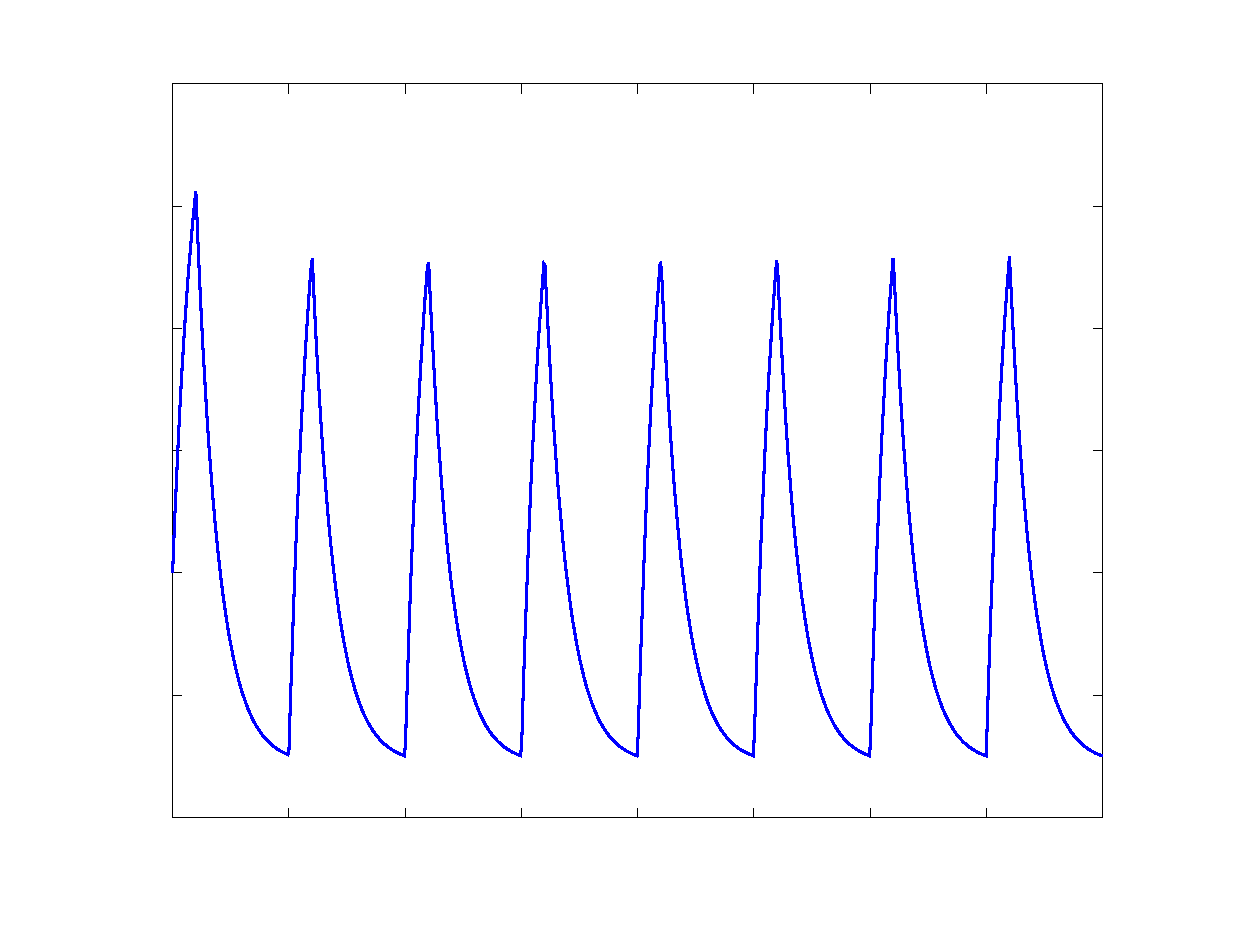
\includegraphics[width=0.8\textwidth]{images/examples/membrane_voltage}}%
    \gplfronttext
  \end{picture}%
\endgroup


\begin{sidewaystable}[ht]


\begin{tabular}{r c l l}
\hline\hline
Current description & Notation & Functional form & Parameter values \\ [0.5ex]
\hline
Background sodium & $I_{\rm Na_b}$ & $\bar{g}_{\rm Na_b} (V_{\rm m} - E_{\rm Na})$ \cite{UNKNOWN}
                          & $\bar{g}_{\rm Na_b} = $ \cite{UNKNOWN}, $E_{\rm Na} = $ \cite{UNKNOWN}\\
Background potassium & $I_{\rm K_b}$ & $\bar{g}_{\rm K_b} (V_{\rm m} - E_{\rm K})$ \cite{UNKNOWN}
                          & $\bar{g}_{\rm K_b} = $ \cite{UNKNOWN}, $E_{\rm K} = $ \cite{UNKNOWN}\\
Sodium-potassium pump & $I_{\rm NaK}$ & $\bar{I}_{\rm NaK}
\frac{[\rm K^{+}]_{\rm c}}{[\rm K^{+}]_{\rm c} + k_{\rm NaK_{K}}}
\frac{[\rm Na^{+}]^{1.5}_{\rm i}}{[\rm Na^{+}]^{1.5}_{\rm i} + k^{1.5}_{\rm
    NaK_{Na}}}
\frac{V + 150}{V + 200}$\cite{Nygrenetal1998} & \cite{Nygrenetal1998}\\
Sodium-calcium exchanger & $I_{\rm NaCa}$ & $k_{\rm NaCa}
\frac{[\rm Na^{+}]^{3}_{i}[\rm Ca^{2+}]_{c} \exp(\frac{\gamma V F}{R T}) -
[\rm Na^{+}]^{3}_{c}[\rm Ca^{2+}]_{i} \exp(\frac{(\gamma - 1.0) V F}{R T})}
{1.0 + d_{\rm NaCa}([\rm Na^{+}]^{3}_{c}[\rm Ca^{2+}]_{i} + [\rm
  Na^{+}]^{3}_{i}[\rm Ca^{2+}]_{c})}$
\cite{Nygrenetal1998} & \cite{Nygrenetal1998}\\
Sodium-hydrogen exchanger & $I_{\rm NaH}$ & \cite{UNKNOWN} & \cite{UNKNOWN}\\
Ultra-rapidly rectifying potassium & $I_{\rm K_{ur}}$ & $g_{\rm
  K_{ur}}\, a_{\rm ur}\, i_{\rm ur}\, (V_{\rm m} - E_{\rm K})$ \cite{Maleckaretal2009} & \cite{Maleckaretal2009}\\
Two-pore potassium channel & $I_{\rm K_{2\, pore}}$ & \cite{UNKNOWN} & \cite{UNKNOWN}\\
Calcium-activated potassium & $I_{\rm Ca_{act}K}$ & \cite{UNKNOWN} & \cite{UNKNOWN}\\
Trip channel(s) & $I_{\rm TRP}$ & $\bar{g}_{\rm NaCa_{TRP}}\, (V_{\rm
  m} - E_{\rm NaCa})$ \cite{UNKNOWN} & \cite{UNKNOWN}\\
Applied stimulus & $ I_{\rm stim}$ & Mirroring experiments \cite{Clarketal2011} &  --- \\ [1ex]
\hline
\end{tabular}
\caption{Details of the model}
\label{table:chondrocyte-model-details}
\end{sidewaystable}

% Local Variables:
% TeX-master: "chondrocyte-model"
% mode: latex
% mode: flyspell
% End:
